\section*{Methodik} % (fold)
\label{sec:methodik}
Zunächst müssen die Transitionen, die in dem Petri-Netz aus Übung 1 erstellt wurden genauer untersucht werden. Jede Transition stellt eine Handlung dar die von einem Koch vollzogen werden kann. Zu jeder Handlung muss überlegt werden wie viel Zeit für sie benötigt wird. Renew bietet eine Verteilungsfunktion an mit der sich Zeiten zufällig bereitstellen lassen. Diese Funktion wird zunächst genauer angeschaut (siehe Abbildung \ref{pic:negexp}).

\begin{figure}[ht]
  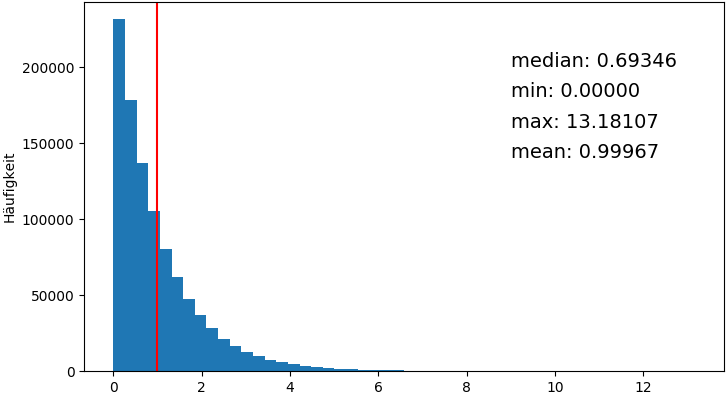
\includegraphics[width=1\textwidth]{pics/negexp.png}
  \caption{Histogramm für die Verteilungsfunktion negexp(1) von Renew nach 1Mio Wiederholungen }
  \label{pic:negexp}
\end{figure}

Wie der Name der Funktion bereits andeutet handelt es sich um eine negativ exponentiell abfallende Funktion. Aus dem gezeigten Graphen lässt sich ablesen das der Eingabewert der Funktion die durchschnittliche Zeit der Ausgabe darstellt. Die Hälfte aller Ausgabewerte ist unter $0.7$ und kompakt auf einer Breite von $0.7$ vertreten, die zweite Hälfte von $0.7$ bis $13.8$ ist wesentlich breiter verteilt mit verschwindend geringer Wahrscheinlichkeit für hohe Werte. 

\begin{figure}[ht]
  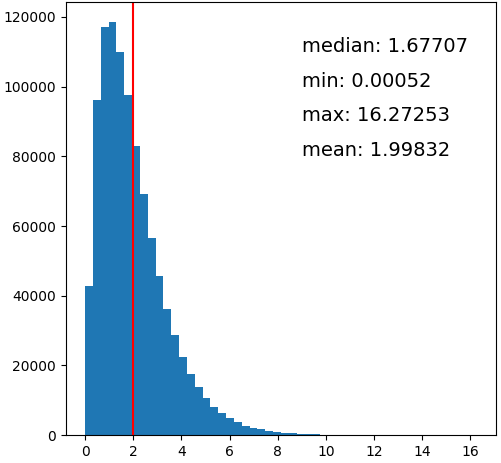
\includegraphics[width=1\textwidth]{pics/negexp2.png}
  \caption{Histogramm für negexp(1) + negexp(1) für 1Mio Wiederholungen}
  \label{pic:negexp2}
\end{figure}

Ähnlich wie bei einem Wurf mehrerer Würfel ergibt sich für die Addition zweiter Funktionsaufrufe ein neuer Peak. Der neue Graph (Abbildung \ref{pic:negexp2}) ist nun nicht mehr konstant fallend sondern steigt zunächst bis auf sein Maximum und fällt danach ab. Ein ähnliches Verhalten wird in der Simulation ebenfalls, bei der Aneinanderreihung der Handlungen der Köche, erwartet. Diese Eigenschaft scheint intuitiv gut geeignet um die Zeit für diesen Prozess zu berechnen da bei der Herstellung eines Gerichtes einerseits Köche verschieden schnell arbeiten, was zunächst für eine Normalverteilung spricht. Allerdings können auch unvorhergesehene Dinge passieren die den Herstellungsprozess stören wie z.B. das sich ein Koch verletzt, Zutaten nicht vorbereitet sind oder ein Koch gerade eine Zigarette rauchen ist. So kann es in Einzelfällen zu wesentlich höheren Herstellungszeiten führen. Mit zunehmender Anzahl von Handlungen wird die Varianz der Zeiten im Verhältnis sinken, denn je mehr Zeiten aufaddiert werden desto geringer ist die Wahrscheinlichkeit das alle Werte sehr hoch oder sehr niedrig werden.

Es muss weiter beachtet werden, dass Handlungen einen minimalen Zeitaufwand haben. Ein Funktionsaufruf von negexp() kann auch einen Wert von 0 zurückliefern und die Handlung so direkt nach Antritt abschließen. Dieses Verhalten ist nicht gewünscht und wird verhindert dadurch, dass eine konstante hinzuaddiert wird, die den minimalen Zeitaufwand darstellt. Eine Zeitfunktion sieht dann wie folgt aus:

\begin{eqnarray}
	t_{tr_i}  = & t_{tr_{i,1}} \cdot Dist.negexp(t_{tr_{i,2}}) & \\
	t_{tr_i,\mu}  = & t_{tr_{i,1}} +t_{tr_{i,2}}  & \textrm{(Durchschnitt)}\\
	\widetilde{t}_{tr_i}  \approx & t_{tr_{i,1}} + 0.69 \cdot t_{tr_{i,2}} & \textrm{(Median)}
\end{eqnarray}



Für die Entwicklung des neuen timed Net's können die Köche als Ressourcen angenommen werden die jeweils nur von einer Transition zur Zeit genutzt werden können. 

Wenn für alle Transitionen Zeiten hinterlegt sind kann mit den Simulationen begonnen werden. Die Simulationen werden dann für 1,2,3,4 und 6 Köche jeweils einige male wiederholt bis sich ein repräsentatives Ergebnis ablesen lässt.












